\documentclass[a4paper, 12pt]{article}

\usepackage{pdfpages}
\usepackage[english]{babel}
\usepackage[left=1.1in, right=1.1in, top=2in, bottom=2in]{geometry}
\usepackage[utf8]{inputenc}
%\usepackage[onehalfspacing]{setspace}
\usepackage{multicol}
\usepackage{hyperref} %to add hyperlinks
\usepackage{diagbox} %to add bifurcating tables
\usepackage{tikz} %to draw diagrams
\usepackage{amsmath, amssymb, amsthm, amsfonts}
%\usepackage{parskip}

\usepackage{xcolor}
\definecolor{light-gray}{gray}{0.92}
\newcommand{\code}[1]{\colorbox{light-gray}{\texttt{#1}}}

\newtheorem{theorem}{Theorem}[section] % index every theorem using sections
\newtheorem{corollary}{Corollary}[theorem]
\newtheorem{lemma}[theorem]{Lemma}
\newtheorem*{definition}{Definition} % don't number the definitions
\theoremstyle{remark} % to make remarks italic instead of bold
\newtheorem*{remark}{Remark}

\renewcommand{\qedsymbol}{$\blacksquare$}

\linespread{1.1} % to set linespacing

\pagestyle{headings}

\usepackage{imakeidx} %to include index
\makeindex

\begin{document}
\includepdf{cover}
\thispagestyle{empty}
\begin{abstract}
	This article investigates the regular games of Nim and Chomp and how they can be generalised to graph nims and graph chomps. These are poset games and they can be analyzed on graphs. Many of the combinatorial games can be studied on graphs. This is the object of this article.\\
\end{abstract}

\clearpage
\thispagestyle{empty}
\begin{center}
	\textbf{Acknowledgements}
\end{center}

I sincerely express my thanks of gratitude to Dr. K.S. Mallikarjuna Rao for supervising me to work on this project. His continued support and guidance made this work possible. I also thank everyone who directly or indirectly helped me in completing this project.\\

\noindent Huidrom Ronald Mangang\\
IISER Mohali\\
September 28, 2021\\

\clearpage

%{\centering \subsection*{Keywords}}
%\begin{center}
%	\textit{nim, chomp, strategy-stealing argument, poset, simplicial complex, bipartite graph, nim-value}
%\end{center}

\thispagestyle{empty}
\tableofcontents
\clearpage


\section{Introduction}

A combinatorial game is a game which is generally played by two or more players, is seqential in that each player involved perform the legal moves alternately, is deterministic in that it does not rely on chance such as tossing a coin or rolling a die, has complete information about the past and present state of the game which is known to all the players. Each player knows the available moves in the game and all the past and present game positions. In combinatorial game theory, we study mostly finite games (that terminate after finitely many moves) and there is always one winner, which is decided according to if the game follows \textit{normal play} or \textit{misere play} (will be defined later). By this strict sense, chess and tic-tac-toe are not combinatorial games for chess can go on infinitely long in theory and may not have a winner while tic-tac-toe may, although finite, also end in a draw. However, we may sometimes treat them as combinatorial games because they mimic combinatorial games in many ways and can be studied using the similar techniques of combinatorial game theory.\\

We shall look at a certain class of combinatorial games known as \textit{poset} games. These games are played on posets or partially ordered sets (will be defined later) and can be studied as games on graphs.\\

In the introduction section, we also define some terminology which we shall be using in the remainder of this paper. In section \ref{preliminaries}, we look into some mathematics and notations that we shall be using. In section \ref{nim}, we discuss the nim game along with Sprague-Grundy theorem, which links nim to other combinatorial games. In section \ref{chomp}, we look at the game of chomp and in section \ref{subsettakeaway}, we discuss the subset take-away game and how it can be studied using graphs and geometry. Section \ref{chompthegraph} deals with a more general version of chomp called the graph chomp. Section \ref{graphnim} looks at a the nim game played on a graph.\\

\noindent We now introduce some terms.
\begin{enumerate}
	\item \textbf{Position}: It is the state of the game at any given time. Every game has a starting position and a terminating postion. A game may have finitely many positions.
	\item \textbf{Move}: Any of the legal and possible options available to a player at any position. A move takes a game position to another.
	\item \textbf{Normal play}: If a game follows this convention, then the player unable to perform a move loses. Unless otherwise stated, we always assume this is the case.
	\item \textbf{Misere play}: The player who performs the final move loses.
	\item \textbf{P-position}: It is a game position in which the player who just moved (\textit{P}revious player) can secure a win. In other words, the player to perform next can be forced to lose. The terminating position is a P-position (for normal play) and an N-position (for misere play).
	\item \textbf{N-position}: It is a game position in which the player who is to move \textit{N}ext can secure a win. In other words, the previous player can be forced to lose.
	\item \textbf{Impartiality}: An impartial game is one in which the legal moves depend only on the position and not on the player who is to make the move. For example, chess is not an impartial game (it is called \textit{partisan}) for a player can only move her own pieces.
	\item \textbf{Winning strategy}: This is the strategy or set of strategies (or moves) which guarantee a win for a player from a game position. If we can find a winning strategy, then we shall say that the game is solved.
\end{enumerate}

\noindent All game positions are either P-positions or N-positions. It can be proven that all positions which are one move away from a P-position are N-positions. Likewise, there is always a move that takes an N-position to a P-position. The rule to win the game is simple --- always leave the game in a P-position (if possible) until the game terminates.

\noindent Unless otherwise stated, we shall assume that every game is impartial, is a two-player game, has finitely many moves, has one winner which is decided by normal play convention.

\section{Preliminaries}
\label{preliminaries}

\subsection{Partially ordered set}
\index{poset}

A \textit{partially ordered set} or \textit{poset} refers to any set $S$ such that for all $a, b, c \in S$ there exists a relation $<$ satisfying the following conditions:
\begin{itemize}
	\item $a \nless b$ whenever $b < a$,
	\item $a < c$ whenever $a<b$ and $b<c$,
	\item $a \nless a$.
\end{itemize}

The subset relationship in the power set of any set makes it a poset as it satisfies all the conditions above. For any poset $(S,<)$, we can define an impartial two-player game in which a legal move is choosing any element $s \in S$ and removing all elements $k \in S$ satisfying $k \leq s$. Such games are known as poset games. Combinatorial games are usually played normally, so the player to remove the last element(s) wins.

\subsection{Abstract simplicial complex}

A \textit{simplex} \index{simplex} in $n$-dimensions (sometimes written as $n$-simplex) is the simplest possible polytope in $n$-dimensions. In one-dimension, it is a line segment. In two-dimensions, it is a triangle. In three-dimensions, it is a tetrahedron and so on. From this, one can infer that an $n$-simplex is a convex envelope of $n+1$ vertices. Simplexes combine to form \textit{simplicial complexes}, which are actually sets that have all simplexes of lower dimensions --- a simplicial $n$-complex includes at least one $n$-simplex and all its constituent simplexes. For a simplicial $3$-complex, it includes a tetrahedron, all its faces which are triangles, all the edges that make up the triangles and all the nodes that make up the edges.\\

An \textit{abstract simplicial complex} \index{simplicial complex} (often denoted by $\Delta$) is the combinatorial counterpart to the geometrical concept of simplicial complex. It is a set-family such that every subset of a set in the family is also in the family. A power set, for instance, is an abstract simplicial complex. The power set of a set of 3 elements, say $A=\{1,2,3\}$, corresponds to the following simplicial 2-complex. Proper subsets of $A$ correspond to the nodes (one-element subsets) and edges (two-element subsets). For a set of 4 elements, the power set corresponds to a simplicial 3-complex (in the form of a tetrahedron).\\

\begin{center}
\begin{tikzpicture}
\draw (0,0) node[anchor=north east]{$2$} -- (1.5,2.6) node[anchor=south]{$1$}-- (3,0) node[anchor=north west]{$3$}-- cycle;
\filldraw[black] (0,0) circle (1.5pt);
\filldraw[black] (1.5,2.6) circle (1.5pt);
\filldraw[black] (3,0) circle (1.5pt);
\end{tikzpicture}\\
\end{center}

If a simplicial complex $\Delta_1$ can be transformed into another simplicial complex $\Delta_2$ just by relabeling the vertices, we say $\Delta_1$ and $\Delta_2$ are \textit{isomorphic} to each other. In the study of the subset take-away game by using simplicial complexes, the labels of the vertices don't really matter.\\

\subsection{Graph}
\index{graph}

In loose terms, a graph is a set of vertices (nodes) and egdes connecting vertices. We represent a graph by $G = (V,E)$ where $V$ and $E$ are the sets of vertices and edges respectively. Degree \index{degree} of a vertex $v \in V$ (written as $deg(v)$) is the number of egdes connected to it.\\

A graph may contain loops and parallel edges. A loop \index{loop} is a vertex connecting to itself (diagram below: left). Parallel edges \index{parallel edge} are multiple edges connecting the same pair of vertices (diagram below: right). A simple graph is one which has no loops or parallel edges. Degree of a vertex is the number of edges it is connected to.\\

\begin{center}
\begin{tikzpicture}
\draw (1.5,0) circle (1.5);
\draw (0,0) node[anchor=west]{$a$};
\filldraw[black] (0,0) circle (1.5pt);

\draw (6,0) node[anchor=east]{$p$}.. controls (7.5, 1) .. (9,0) node[anchor=west]{$q$};
\draw (6,0) .. controls (7.5,-1) .. (9,0);
\filldraw[black] (6,0) circle (1.5pt);
\filldraw[black] (9,0) circle (1.5pt);
\end{tikzpicture}\\
\end{center}

A \textit{bipartite graph} \index{bipartite graph} is a simple graph which can be decomposed into two distinct sets of nodes such that no nodes in the same set are connected and every edge in the graph connects two nodes from different sets (diagram below: left). If every node in each set is connected to every node in the other, it becomes a complete bipartite graph (diagram below: right). The maximum number of edges in a complete bipartite graph occur when each set consists of equal number of nodes.\\

\begin{center}
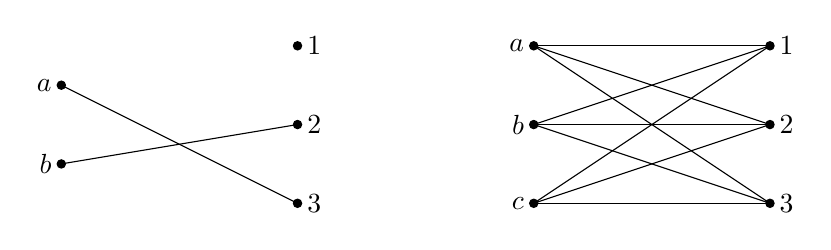
\begin{tikzpicture}
\draw (0, 0.5) node[anchor=east]{$a$} -- (3, -1) node[anchor=west]{$3$};
\draw (0,-0.5) node[anchor=east]{$b$} -- (3, 0) node[anchor=west]{$2$};
\filldraw[black] (0, 0.5) circle (1.5pt);
\filldraw[black] (0,-0.5) circle (1.5pt);
\filldraw[black] (3,0) circle (1.5pt);
\filldraw[black] (3,1) node[anchor=west]{$1$} circle (1.5pt);
\filldraw[black] (3,-1) circle (1.5pt);

\draw (6, 1) node[anchor=east]{$a$} -- (9, 1) node[anchor=west]{$1$};
\draw (6, 0) node[anchor=east]{$b$} -- (9, 0) node[anchor=west]{$2$};
\draw (6,-1) node[anchor=east]{$c$} -- (9,-1) node[anchor=west]{$3$};
\draw (6, 1) -- (9, 0);
\draw (6, 1) -- (9,-1);
\draw (6, 0) -- (9, 1);
\draw (6, 0) -- (9,-1);
\draw (6,-1) -- (9, 1);
\draw (6,-1) -- (9,0);

\filldraw[black] (6, 1) circle(1.5pt);
\filldraw[black] (6, 0) circle(1.5pt);
\filldraw[black] (6,-1) circle(1.5pt);
\filldraw[black] (9, 1) circle(1.5pt);
\filldraw[black] (9, 0) circle(1.5pt);
\filldraw[black] (9,-1) circle(1.5pt);
\end{tikzpicture}\\
\end{center}

A graph is said to be \textit{connected} \index{connected graph} if there is always a path between any pair of vertices, otherwise it is said to be \textit{disconnected}. In the above, the graph on the right is connected while the graph on the left is disconnected as the vertex 1 is isolated.

\begin{definition}
	A path graph \index{path graph} $P_n$ is a graph having $n$ vertices and $n-1$ edges such that there are 2 terminal vertices (degree 1) and all other vertices (if any) have degree 2.
\end{definition}

A path graph is one of the simplest graphs one can draw. There is only one path between any pair of vertices. The following is the path graph of 5 vertices, referred to as $P_5$. The shape do not matter. It can be curvy or any shape so long as it does not violate the essence of a path.\\

\begin{center}
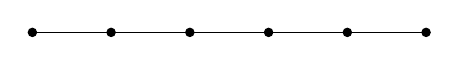
\begin{tikzpicture}
	\draw (0,0) -- (1,0) -- (2,0) -- (3,0) -- (4,0) -- (5,0);
	\filldraw[black] (0,0) circle(1.5pt);
	\filldraw[black] (1,0) circle(1.5pt);
	\filldraw[black] (2,0) circle(1.5pt);
	\filldraw[black] (3,0) circle(1.5pt);
	\filldraw[black] (4,0) circle(1.5pt);
	\filldraw[black] (5,0) circle(1.5pt);
\end{tikzpicture}\\
\end{center}

It is interesting to see that every path graph is a bipartite graph. For instance, the above path $P_5$ can be re-drawn as the following bipartite graph.\\

\begin{center}
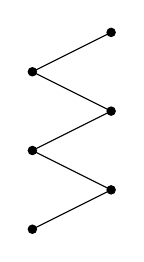
\begin{tikzpicture}
	\draw (0,0) -- (1,0.5) -- (0,1) -- (1,1.5) -- (0,2) -- (1,2.5);
	\filldraw[black] (0,0) circle(1.5pt);
	\filldraw[black] (1,0.5) circle(1.5pt);
	\filldraw[black] (0,1) circle(1.5pt);
	\filldraw[black] (1,1.5) circle(1.5pt);
	\filldraw[black] (0,2) circle(1.5pt);
	\filldraw[black] (1,2.5) circle(1.5pt);
\end{tikzpicture}\\
\end{center}

\begin{definition}
	A $k$-regular graph \index{regular graph} is a graph in which every vertex has the same degree $k$.
\end{definition}

We shall use the notation $^k R_n$ to represent a $k$-regular graph of $n$ vertices. So, $^2 R_3$ is a triangle, $^2 R_4$ is a quadrilateral and so on. In short, $^2 R_n$ is an $n$-gon. There may be multiple forms of $^k R_n$ for same $k$ and $n$. For instance, the following is a $3$-regular graph with $6$ vertices. But we can also draw in the form of a hexagon and connect the opposite vertices.\\

\begin{center}
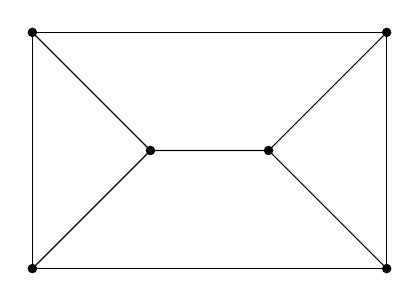
\begin{tikzpicture}
	\draw (0,0) -- (4.5,0) -- (4.5,3) -- (0,3) -- cycle;
	\draw (0,0) -- (1.5,1.5) -- (3,1.5) -- (4.5,3);
	\draw (0,3) -- (1.5,1.5);
	\draw (3,1.5) -- (4.5,0);
	\filldraw[black] (0,0) circle(1.5pt);
	\filldraw[black] (4.5,0) circle(1.5pt);
	\filldraw[black] (4.5,3) circle(1.5pt);
	\filldraw[black] (0,3) circle(1.5pt);
	\filldraw[black] (1.5,1.5) circle(1.5pt);
	\filldraw[black] (3,1.5) circle(1.5pt);
\end{tikzpicture}\\
\end{center}

	Edges can have directions (accomplished by putting an arrow on it, like vectors). Graphs that consist of such edges are said to be \textit{directed} \index{directed graph}. An undirected graph has no such vector-like edges --- only vertices and edges and no sense of direction. 

\begin{definition}
	A tree \index{tree} is an undirected graph in which any pair of vertices is connected by exactly one path. A forest \index{forest} is a disjoint union of trees.
\end{definition}

Trees look like trees and forests, as usual, is just a group of trees such that no two trees are connected. Given below is a forest that has three trees.\\
	
\begin{center}
\begin{tikzpicture}
	\draw (0,0) -- (0,1) -- (0.707,1.707) -- (0.707,2.707) -- (1.414,3.314);
	\draw (0,1) -- (-0.707,1.707);
	\draw (0.707,2.707) -- (0,3.314);
	
	\filldraw[black] (0,0) circle(1.5pt);
	\filldraw[black] ([xshift=-2pt,yshift=-2pt]0,1) rectangle ++(4pt,4pt);
	\filldraw[black] (0.707,1.707) circle(1.5pt);
	\filldraw[black] (-0.707,1.707) circle(1.5pt);
	\filldraw[black] ([xshift=-2pt,yshift=-2pt]0.707,2.707) rectangle ++(4pt,4pt);
	\filldraw[black] (1.414,3.314) circle(1.5pt);
	\filldraw[black] (0,3.314) circle(1.5pt);
	
	\draw (3,0) -- (3.707,0.707) -- (4.414,0);
	\draw (3.707,0.707) -- (3.707,1.707) -- (4.414,2.414) -- (4.414,3.414);
	\draw (3.707,1.707) -- (3,2.414);
	
	\filldraw[black] (3,0) circle(1.5pt);
	\filldraw[black] (4.414,0) circle(1.5pt);
	\filldraw[black] ([xshift=-2pt,yshift=-2pt]3.707,0.707) rectangle ++(4pt,4pt);
	\filldraw[black] (3.707,1.707) circle(1.5pt);
	\filldraw[black] ([xshift=-2pt,yshift=-2pt]4.414,2.414) rectangle ++(4pt,4pt);
	\filldraw[black] ([xshift=-2pt,yshift=-2pt]3,2.414) rectangle ++(4pt,4pt);
	\filldraw[black] (4.414,3.414) circle(1.5pt);
	
	\draw (7,0) -- (6.29,0.707) -- (6.29,1.707);
	\draw (7,0) -- (7.707,0.707) -- (7.707,1.707) -- (8.414,2.414);
	
	\filldraw[black] (7,0) circle(1.5pt);
	\filldraw[black] ([xshift=-2pt,yshift=-2pt]6.29,0.707) rectangle ++(4pt,4pt);
	\filldraw[black] (6.29,1.707) circle(1.5pt);
	\filldraw[black] ([xshift=-2pt,yshift=-2pt]7.707,0.707) rectangle ++(4pt,4pt);
	\filldraw[black] (7.707,1.707) circle(1.5pt);
	\filldraw[black] ([xshift=-2pt,yshift=-2pt]8.414,2.414) rectangle ++(4pt,4pt);
\end{tikzpicture}\\
\end{center}

	There is nothing special about the square and circular dots on the vertices. It is put that way just to illustrate that all vertices of a tree can be grouped into two sets such that no two vertices in the same set are connected by an edge. In other words, every tree is a bipartite graph. Also, every path graph is a tree.
	
\begin{remark}
	To decompose $V$ of a tree into a bipartite graph of sets $A$ and $B$, one can simply start by putting a terminating vertex into set $A$. All vertices adjacent to this vertex are put in set $B$. All vertices adjacent to the vertices of set $B$ are put in set $A$ and so on, until all vertices in $V$ are exhausted.
\end{remark}


We shall use the EV parity system \index{EV parity}: each graph has a value denoted by $(e,v)$ where $e=0$ if there are even number of edges, otherwise $e=1$ and the same applies for $v$, which denotes vertices (nodes). This implies that each graph has an EV parity which belongs to the set $\{(0,0), (0,1), (1,0), (1,1)\}$.

\section{Nim}
\label{nim}
\index{nim}

In the game of Nim, there are a number of heaps and a number of counters in each heap. The legal moveset is simple - a player may remove any number of counters from a heap. She has to remove at least one counter and may not remove from more than a heap at once. The player unable to perform a move loses (normal play). For example, we choose the following configuration - four heaps with two, three, four and five counters in each. A particular route of the game is given below.\\
 
\noindent \hspace*{0.8in}\code{P Q R S}\\
\noindent \hspace*{0.8in}\code{2 3 4 5}\hspace*{0.8in} \code{Player A removes 2 from Heap P.}\\
\noindent \hspace*{0.8in}\code{0 3 4 5}\hspace*{0.8in} \code{Player B removes 2 from Heap Q.}\\
\noindent \hspace*{0.8in}\code{0 1 4 5}\hspace*{0.8in} \code{Player A removes 1 from Heap S.}\\
\noindent \hspace*{0.8in}\code{0 1 4 4}\hspace*{0.8in} \code{Player B removes 1 from Heap Q.}\\
\noindent \hspace*{0.8in}\code{0 0 4 4}\hspace*{0.8in} \code{Player A removes 2 from Heap R.}\\
\noindent \hspace*{0.8in}\code{0 0 2 4}\hspace*{0.8in} \code{Player B removes 2 from Heap S.}\\
\noindent \hspace*{0.8in}\code{0 0 2 2}\hspace*{0.8in} \code{Player A removes 1 from Heap S.}\\
\noindent \hspace*{0.8in}\code{0 0 2 1}\hspace*{0.8in} \code{Player B removes 1 from Heap R.}\\
\noindent \hspace*{0.8in}\code{0 0 1 1}\hspace*{0.8in} \code{Player A removes 1 from Heap S.}\\
\noindent \hspace*{0.8in}\code{0 0 1 0}\hspace*{0.8in} \code{Player B removes 1 from Heap R.}\\
\noindent \hspace*{0.8in}\code{0 0 0 0}\hspace*{0.8in} \code{Player A has no move left; Player B wins.}\\

We ask this question: is there a winning strategy for a given configuration of heaps and counters? In other words, is there a set of moves defined by a rule such that it guarantees a win for a player? We shall attempt to answer this question. The position \code{0 0 0 0} is said to be P-position as the next player cannot perform a move. The position \code{0 0 1 1} is also a P-position as the next player is forced to take 1 from any of the non-empty heaps such that she loses. The position \code{0 0 0 n} is an N-position as the next player can take the last heap. We shall need some arithmetic for our purpose. The XOR operation, for instance, operates on binary numbers --- it adds them bit by bit without carrying. An odd number of 1s give 1; an even number of 1s give 0. For two operands, this means $1+1=0$, $0+1=1$, $1+0=1$ and $0+0=0$. For three operands, $1+1+1 = 1$, $1+1+0=0$, $1+0+0=1$, $0+0+0=0$ and so on. Given two binary numbers 111 and 101, we can do XOR operation as $111\oplus101=010$ (we perfomed XOR bit by bit). The symbol $\oplus$ is used for such operation. We shall now define an important term that we shall be using quite often.\\

\noindent \textbf{Nim-sum} \index{nim-sum}: The XOR of all heap sizes at a given position.\\

For the configuration \code{2 3 4 5}, we have $010+011+100+101=000$, which means \code{2 3 4 5} has nim-sum of $0$. Similarly, \code{0 0 1 1} and \code{0 0 0 0} has nim-sums of $0$. These are P-positions. In fact, it can be proven that any position which has nim-sum $0$ is a P-position. The winning strategy is then to finish every move with a nim-sum of $0$. We shall now look into two important lemmas.

\begin{lemma}
	If a position has Nim-sum of $0$, the next move changes it to some non-zero value.
\end{lemma}

\noindent We can show this. Consider a position \code{$x_1$ $x_2$ $x_3$ ... $x_n$}. We have the nim-sum $s = x_1\oplus x_2\oplus x_3\oplus ... \oplus x_n$. Suppose after a move we have the position \code{$y_1$ $y_2$ $y_3$ ... $y_n$} and nim-sum $t = y_1\oplus y_2\oplus y_3\oplus ... \oplus y_n$. Suppose $s=0$. Since only one heap can be modified after a move, we have $x_k \ne y_k$ for some $k$ and $x_i = y_i$ for $i \ne k$. We have:\\

\noindent $t = t \oplus 0$\\
\hspace*{0.28cm}$=t \oplus s \oplus s$ \\
\hspace*{0.28cm}$= (y_1\oplus y_2\oplus y_3\oplus ... y_n)\oplus(x_1\oplus x_2\oplus x_3\oplus ... \oplus x_n)\oplus s $\\
\hspace*{0.28cm}$= (y_1\oplus x_1)\oplus(y_2\oplus x_2)\oplus (y_3\oplus x_3)\oplus ... \oplus(y_k\oplus x_k)\oplus s$\\
\hspace*{0.28cm}$= y_k \oplus x_k \oplus s$\\

\noindent $y_k \oplus x_k$ will never be zero; and if $s=0$, then $t \ne 0$. This means if a player makes the nim-sum $0$ in her turn, the other player must make it non-zero.

\begin{lemma}
	If a position has a Nim-sum of non-zero value, it is always possible to make it zero by the next move.
\end{lemma}

\noindent Choose a heap $x_k$ such that its most significant bit is in the same position as that of the most significant bit in $s$. For instance, given a game-position \code{2 3 4}, we choose the third heap which has binary value 100. Its most significant bit is in the same position as that of the most significant bit in the nim-sum 101 (since $10\oplus 11 \oplus 100 = 101$). Make the new value of the heap $y_k = s\oplus x_k$ by removing $x_k - y_k$ counters from the heap. The new nim-sum will be:\\

\noindent $t =  y_k \oplus x_k \oplus s$ (from above)\\
\hspace*{0.28cm}$= s\oplus x_k\oplus x_k \oplus s$\\
\hspace*{0.28cm}$= 0$\\

\noindent In the example we considered above, we could remove $4-1$ counters from the third heap such that we get the game-position \code{2 3 1} which has nim-sum of $0$. We shall now have the following theorem.

\begin{theorem}
	Any position which has Nim-sum of 0 is a P-position.
\end{theorem}

\begin{proof}
	Suppose a player makes her move such that she leaves a nim-sum of $0$. Then the opponent always disturbs the nim-sum (lemma 1) to some non-zero value. But by lemma 2, she can always make her move to leave a nim-sum of $0$. Her strategy is now to always set the nim-sum to $0$ at her turn. This can continue until she can finish the game with \code{0 0 ... 0} which has a nim-sum of $0$, which leaves her the winner. Had she started the game from nim-sum of $0$, she would have no choice but to disturb the nim-sum to some non-zero value. Her only option would be then to hope that her opponent makes a mistake in his move such that she could bring the nim-sum to $0$ and turn the tide in her favour. We now see that there is a winning strategy for the game of Nim, but which player has it depends on the starting position. We have now proven that any nim position in which the nim-sum is zero is a P-position, else the position is an N-position.
\end{proof}

Any position in a two-player impartial game (like nim) corresponds to a heap of $n$ counters, where the number $n$ is called the nim-value (or Sprague-Grundy number)\index{Grundy number} of that position. This is the Sprague-Grundy \index{Sprague-Grundy theorem} theorem.\\

A nim-value of 0 implies the heap is empty, which means the player who has just performed a move has won as there are no moves left. This is called a P-position, because the \textit{p}revious player wins. Any non-zero nim-value implies the heap is non-empty, which means the \textit{n}ext player to perform a move wins by taking all counters. This is called an N-position. Any game position of zero nim-value is a P-position, otherwise an N-position.\\

The nim-value of a game is given by the \textit{mex} rule. The \textit{m}inimum \textit{ex}cluded value or \textit{mex} \index{mex rule} of a set is the minimum non-negative integer excluded from the set --- this means mex$\{1,3,5,7\}=0$ and mex$\{0,1,3,7\}=2$. The nim-value $\gamma(\tau)$ of a game position $\tau$ is the mex of nim-values the next player can move to from $\tau$ --- that is, $\gamma(\tau)=$ mex$\{\gamma(\tau_1), \gamma(\tau_2), .., \gamma(\tau_n) \}$, where $\tau_i$'s are the possible game positions obtainable by one move from $\tau$.\\

If $\gamma(\tau)=0$, it is a P-position as stated earlier. The next move should shift the nim-value to some nonzero value, which is an N-position. There is always a move to bring the nim-value back to zero. This implies that a P-position is always followed by an N-position by the next move, which can then be brought back to P-position. Therefore, if we can determine all P-positions and N-positions of a game, we have determined the winning strategy, for the player facing an N-position can always give his opponent a P-position, so that he receives an N-position in return. Since the game is finite, this continues until the winning player eventually moves to an ending P-position from which the opponent has no legal move available to him.

\section{Chomp}
\label{chomp}
\index{chomp}

In the common version of the Chomp, which is also known as two-dimensional chomp or 2D chomp, there is a rectangular grid in which the bottom left square is poisoned. Two players alternate in making moves and each move consists of taking out any square from the grid including all squares that lie above and right to the one which is picked. In other words, if we number each square with a pair of coordinates such that the poisoned square is $(1,1)$, then a move consists of picking a square $(h,k)$ including all squares $(x,y)$ such that $x \geq h$ and $y \geq k$. The player who takes the poisoned square loses. It is easily seen that the game can be extended to the trivial one-dimensional case and to higher dimensions. For one-dimensional case, we can easily use one integer coordinate for each square and one move would mean taking out a square $h$ and all squares $x$ such as $x \geq h$. For three-dimensional case, a move will be taking out a square $(h, k, l)$ and all squares $(x, y, z)$ such that $x \geq h$, $y \geq k$ and $z \geq l$. We shall now look into the strategy-stealing argument, which is often helpful in proving the non-existence of a winning strategy for the second player.\\

\noindent \textbf{Strategy-stealing argument} \index{strategy-stealing}: It relies on building a contradiction. It is assumed that the second player has a winning strategy, which means he can always force a win no matter which move the first player performs. After an arbitrary first move, the first player may use the winning strategy (if possible) in response to any move by the second player. This means that both the players have winning strategy --- which is impossible, and hence contradicts the assumption that such a strategy exists.\\

There are many instances where we can use the strategy-stealing argument to prove that the second player has no winning strategy. We shall be using it to prove the following theorem.

\begin{theorem}
	In the game of Chomp, the first player has a winning strategy.
\end{theorem}

\begin{proof}
	Consider a rectangular grid of size $m\times n$. Suppose the first player picks the square $(m,n)$. Assume the second player has a winning strategy and he uses it to perform a move, say $(h,k)$. This guarantees him a win. However, the first player could have started with the square $(h,k)$ and then use the winning strategy to guarantee herself a win. This contradicts the assumption that the second player has a winning strategy and hence he does not have one. This means that there is always a move for the first player such that the second player has no move to ensure a second player win. Since the game must terminate after a finite number of moves, the first player can always win.
\end{proof}

On paper, the first player can win but in practice, it is not as easy as it might look. We only proved that a winning strategy exists for the first player but we do not know what it is. For small values of $m$ and $n$, a computer can calculate all possible moves such that we might lose even if we are the first player. It is very hard to write down a first player winning strategy for a general $m \times n$ grid even if we know it exists! But for some special cases, we can do it.\\

For a $n \times n$ grid where $n>1$, we can write down the winning strategy for the first player. The idea is to always keep the grid in symmetry down to the last square, thus forcing the second player to take the poisoned square. To keep the grid in symmetry, we can take any of the squares that lie on the diagonal, viz., $(2,2), (3,3), ... ,(n,n)$. Although picking any of these squares will keep the symmetry, it does not make much sense to take $(n,n)$ because the second player can take any one of the other diagonal squares, thus stealing our strategy to guarantee himself a win. Our goal is to force him to break symmetry while we restore symmetry at every turn. Thus, we are left with only one option, viz., $(2,2)$. Taking $(2,2)$ should be then the first move for the first player. The second player is then forced to take only squares $(1, k)$ or $(h, 1)$. Suppose he takes $(1, k)$. Then the first player can take $(k,1)$ and restore symmetry. From this position, no matter which square he takes, the first player can always peform a similar move to restore symmetry. This continues until he is forced to take the poisoned square. Thus, the first player wins.\\

For a $n\times 2$ grid ($n$ columns and two rows) where $n>1$, the first player starts by removing the square at the top-right corner, viz., $(n,2)$. The idea is to keep the grid always like this --- the top row shorter than the bottom row by one square. If she can do this at every turn, she will eventually leave the poisoned square for the second player to take and lose. After the top-right square is removed, the second player has two choices --- to remove from the top row or the bottom row. Suppose he removes from the top row, say $(h,2)$. She can then remove $(h+1,1)$ so that she leaves the top row shorter than the bottom row by one square. If he removes from the bottom row, then she can remove the top-right square to leave it in her preferred position. As the game goes on, the columns become shorter. If the first player does not mess up, she can force a win by leaving only the poisoned square. Thus we have arrived at a winning strategy for the $n\times 2$ type. Suppose the first player has messed up at certain point, say starting her first move with a square other than the top-right one. Then the second player can use the same winning strategy outlined above to guarantee himself a win. Thus if the first player does not take the top-right square, the second player has a winning strategy. Also if she messes up at any position, the second player can always force a win.\\

Due to symmetry, the winning strategy in a $2 \times n$ grid (2 columns and $n$ rows) where $n>1$ is similar to the above. The first player starts by taking the square at the top-right corner, viz., $(2,n)$ and then to keep the right column always shorter than the left column by a square. As in above, this guarantees her a win unless she messes up and gives away the winning strategy to her opponent.\\

Although it's difficult to write down an explicit strategy the general case of $m \times n$ grid, we see that if we can somehow reduce it to the case of $n\times n$ or $n\times 2$ or $2\times n$, then we know we have a winning strategy.

\section{Subset take-away}
\label{subsettakeaway}
\index{subset take-away}

Subset take-away is a poset \index{poset} game played on a super set. For any non-empty finite set $A$, each player take turns in choosing a proper subset of $A$ and removing all its supersets including itself. A player may not choose the empty subset. As in normal play, the player to remove the last subset(s) wins. For instance, if $A = \{1\}$, the rules of the game prevents players from choosing any subset thus rendering the second player the winner. If $A = \{1, 2\}$, there are only two choices available --- either $\{1\}$ or $\{2\}$. The first player chooses one of them and the second player takes the other, thus winning the game. If $A = \{1, 2, 3\}$, the first player can take either a singleton subset of two-element subset. Regardless, the second player can choose its complement, reduce it to the case of 2-element set and force a win. Thus, upto sets of three elements, it is trivial to see that subset take-away is a second-player win. In fact, David Gale went far to make a conjecture \index{David Gale's conjecture} that it is always a second-player win for any finite set.\\

The game can be studied using simplicial complexes \index{simplicial complex}. For a starting $n$-set, we choose $(n-1)$-simplex. A move consists of choosing an element (simplex of lower dimension) and removing all its interior as well as all higher-dimensional simplexes containing it, including itself. For instance, if $A = \{1, 2, 3\}$, we choose 2-simplex (triangle). If the first player takes $\{1,2\}$, then the side 12 is removed leaving 231. As discussed above, the second player can take $\{3\}$, thus removing 3 as well as the sides 23 and 31. Only the nodes 1 and 2 remain, which the first player takes one and the second player takes the remaining node and win.\\

\begin{center}
\begin{tikzpicture}
\draw (0,0) node[anchor=north east]{$2$} -- (1.5,2.6) node[anchor=south]{$1$}-- (3,0) node[anchor=north west]{$3$}-- cycle;
\filldraw[black] (0,0) circle (1.5pt);
\filldraw[black] (1.5,2.6) circle (1.5pt);
\filldraw[black] (3,0) circle (1.5pt);

\draw (5,0) node[anchor=north east]{$2$} -- (8,0) node[anchor=north west]{$3$}-- (6.5,2.6) node[anchor=south]{$1$};
\filldraw[black] (5,0) circle (1.5pt);
\filldraw[black] (8,0) circle (1.5pt);
\filldraw[black] (6.5,2.6) circle (1.5pt);

\filldraw[black] (10,0) node[anchor=north east]{$2$} circle (1.5pt);
\filldraw[black] (11.5,2.6) node[anchor=south]{$1$} circle (1.5pt);
\end{tikzpicture}\\
\end{center}

If $A=\{1,2,3,4\}$, we choose a hollow tetrahedron. Taking a node would mean removing the node, all sides connected to the note, all faces (triangles) that contain the node. Suppose player 1 starts by choosing the edge 13, then faces 123 and 134 are removed as well as the edge 13. The resulting position is given in the diagram below. Player 2 takes the edge 24, removing it as well as faces 124 and 234, leaving just the cyclic graph 1234. Player 1 takes 4, leaving path-graph 123, including nodes 1 and 3. Player 2 takes 2, leaving only the nodes 1 and 3, thus forcing a win.\\

\begin{center}
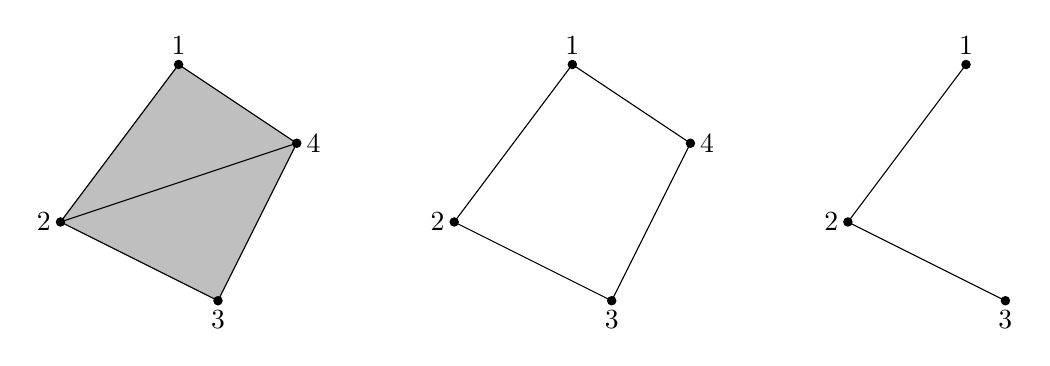
\begin{tikzpicture}
\filldraw[gray!50] (0,0) -- (2,-1) -- (3,1);
\filldraw[gray!50] (3,1)-- (1.5,2) -- (0,0);
\filldraw[black] (0,0) circle (1.5pt);
\filldraw[black] (2,-1) circle (1.5pt);
\filldraw[black] (3,1) circle (1.5pt);;
\filldraw[black] (1.5,2) circle (1.5pt);
\draw (0,0) node[anchor=east]{$2$} -- (2,-1) node[anchor=north]{$3$} -- (3,1) node[anchor=west]{$4$} -- (1.5,2) node[anchor=south]{$1$} -- (0,0) -- (3,1);

\draw (5,0) node[anchor=east]{$2$} -- (7,-1) node[anchor=north]{$3$} -- (8,1) node[anchor=west]{$4$} -- (6.5,2) node[anchor=south]{$1$} -- cycle;
\filldraw[black] (5,0) circle (1.5pt);
\filldraw[black] (7,-1) circle (1.5pt);
\filldraw[black] (8,1) circle (1.5pt);
\filldraw[black] (6.5,2) circle (1.5pt);

\draw (11.5,2) node[anchor=south]{$1$} -- (10,0) node[anchor=east]{$2$} -- (12,-1) node[anchor=north]{$3$};
\filldraw[black] (12,-1) circle (1.5pt);
\filldraw[black] (10,0) circle (1.5pt);
\filldraw[black] (11.5,2) circle (1.5pt);
\end{tikzpicture}\\
\end{center}

A complicated game position may be reduced to a simpler one (if symmetry permits) without affecting its win/loss information. Consider a pair $(x,y)$ of vertcies in a simplicial complex $\Delta$. Suppose there is no edge in $\Delta$ connecting $x$ and $y$. Also suppose $x$ and $y$ are equivalent with respect to $\Delta$ in that for every set $X \in \Delta$ that contains $x$, there is a set $Y \in \Delta$ which is exactly the same as $X$ except it contains $y$ instead of $x$. The same holds if $x$ and $y$ are interchanged. We shall call such a pair $(x,y)$ a \textit{binary star}.

\begin{theorem}
	\label{binarystartheorem}
	If a binary star $(x,y)$ is removed from a simplicial complex $\Delta_1$ along with all the simplices that containing them, the resulting simplicial complex (say $\Delta_2$) has the same win/loss situation as $\Delta_1$. 
\end{theorem}

\begin{proof}
	Consider a binary star $(x,y) \in \Delta_1$. Suppose $\Delta_2$ is the reduced simplicial complex. Suppose Player A has a winning strategy in $\Delta_2$. If Player B makes a move which does not involve either $x$ or $y$, Player A can play according to his winning strategy. If Player B's move involves $x$ (or $y$), Player A can respond by performing the corresponding move involving $y$ (or $x$). This implies all moves involving $x$ or $y$ are stalling moves and $\Delta_1$ can safely be reduced to $\Delta_2$ without affecting win/loss situation.
\end{proof}

Let us look at $A = \{1,2,3,4\}$ again. Player 1 has four moves available to him --- removing a vertex, or edge, or triangle. Removing a vertex (say $4$) leaves the triangle 123. Player 2 can remove 123 (the face) and force a win. Removing an edge (say $12$) leaves a position where $(1,2)$ is a binary pair. By theorem \ref{binarystartheorem}, this can be reduced to the 1-simplex ($34$), which is a Player 2 win. Removing a triangle (face) (say $123$) leaves the following position. Player 2 can remove the vertex 4 and force a win. Thus, for $n=4$, it is a second player win.\\

\begin{center}
	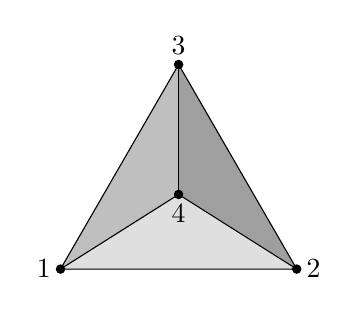
\begin{tikzpicture}
	\filldraw[gray!50] (0,0) -- (1.5,0.948) -- (1.5,2.598);
	\filldraw[gray!75] (3,0) -- (1.5,0.948) -- (1.5,2.598);
	\filldraw[gray!25] (0,0) -- (3,0) -- (1.5,0.948);
	
	
	\draw (0,0) node[anchor=east]{$1$} -- (3,0) node[anchor=west]{$2$} -- (1.5,2.598) node[anchor=south]{$3$} -- cycle;
	\draw (0,0) -- (1.5,0.948) node[anchor=north]{$4$} -- (3,0);
	\draw (1.5,0.948) -- (1.5,2.598);
	
	
	\filldraw[black] (0,0) circle (1.5pt);
	\filldraw[black] (3,0) circle (1.5pt);
	\filldraw[black] (1.5,2.598) circle (1.5pt);
	\filldraw[black] (1.5,0.948) circle (1.5pt);
	\end{tikzpicture}\\
\end{center}

\section{Chomp the Graph}
\label{chompthegraph}
\index{graph chomp}

\subsection{EV parity}

Chomp the Graph is a finite, two-player impartial game where each player take turns in removing an edge or a vertex including the adjacent edges in a graph. As with normal play, the player to perform the last move wins. This game can be considered a special case of the subset take-away where a player may remove only one-element or two-element subsets. Following EV parity system, \index{EV parity} a graph has the parity $(e,v)$, where $e=0$ if $|E|$ is even and $e=1$ if $|E|$ is odd and the same goes for $v$ for the number of vertices. For instance, a graph which has an odd number of edges and even number of vertices has the partiy $(1,0)$.\\

Chomping a path $P_n$ is a trivial case. If $n$ is odd, the first player may remove the middle edge, thus leaving two paths of equal sizes, which is essentially a P-position. If $n$ is even, she may remove the middle edge, which also results in two paths of equal sizes. Therefore, the winning strategy is to always leave the game position in symmetry or two paths of equal sizes, and since the game is finite, it must terminate with the first player winning.\\

It is interesting to see that there is a simple and elegant mapping from any bipartite graph to its Grundy value or nim-value. For any bipartite graph of EV parity $(e,v)$, the binary number $(ev)_2$ gives its nim-value \cite{broadScientific}. This result is summarized in the table below. This essentially implies every bipartite graph with even number of vertices and edges is a P-position, otherwise an N-position. Furthur, there is always a move that takes $p \in \{(0,1),(1,0),(1,1)\}$ to $(0,0)$ and there is no move that takes a $(0,0)$ graph to another $(0,0)$ graph --- thus we have a winning strategy (given below) \cite{broadScientific}. \\

\noindent\textit{Winning strategy for bipartite graph chomp.} For $(0,1)$ graphs, remove a vertex of even degree to make it $(0,0)$, which is always possible \cite{broadScientific}. For $(1,0)$ graphs, removing a edge leaves $(0,0)$. For $(1,1)$ graphs, remove a vertex of odd degree to make it $(0,0)$.

\begingroup
\setlength{\tabcolsep}{8pt}
\renewcommand{\arraystretch}{1.5}
\begin{table}
	\begin{center}
		\caption{\textit{Nim-values for a bipartite graph}}
		\vspace*{0.2cm}
		\begin{tabular}{| l | c| c |}
			\hline
			\diagbox{Edges}{Vertices} & Even & Odd\\
			\hline
			Even & $0$ & $2$\\
			\hline
			Odd & $1$ & $3$\\
			\hline
		\end{tabular}
	\end{center}
\end{table}
\endgroup

\subsection{Computing Grundy numbers}

We shall use the term \textit{follower} for all game positions that follow the game position in hand. The most general way to compute nim-value (Grundy number) of a game position is to list out all its followers and take the minimum excluded value or mex of their nim-values. This can be done in hand for small game positions whose followers are simple and whose nim-values are easily computable. Consider $P_1$ whose followers are a vertex (nim-value $1$) and two vertices (nim-value $0$). Since, mex$(\{0,1\})= 2$, $P_1$ has a nim-value of $2$. Consider $P_2$ whose followers are $P_1$ (nim-value $2$), a vertex and $P_1$ (nim-value $3$) and two vertices (nim-value $0$). Therefore, $P_2$ has a nim-value of $1$. For instance, $P_3$, $P_5$ and all paths of odd number of edges have the nim-value $2$ while all paths of even number of egdes have nim-value of $1$. This leads us to the following theorem.

\begin{theorem}
	\label{nimValueTheoremForPaths}
	A path $P_n$ has nim-value $1$ or $2$ according to whether $n$ is even or odd.
\end{theorem}

\begin{proof}
	Any path $P_n$ is a bipartite graph since all the vertices can alternately be grouped into two disjoint sets such that no pair of vertices in the same set are connected by an edge. This limits its possible nim-values to $\{0,1,2,3\}$ which is decided by its EV parity. If $n$ is even, then the number of vertices is odd, so its nim-value is $(01)_2$ or $1$. Similarly, the nim-value is $2$ when $n$ is odd.
\end{proof}

Theorem \ref{nimValueTheoremForPaths} is an elementary but interesting result, since we can use it to compute nim-values of more complex graphs whose followers are paths. It also directly leads to the following collolary.

\begin{corollary}
	All $2$-regular graphs are P-positions.
\end{corollary}

\begin{proof}
	Every follower of a $2$-regular graph is a path graph, which has a nim-value in $\{1,2\}$. By mex rule, the nim-value of the regular graph is $0$, and hence a P-position.
\end{proof}

In loose terms, a \textit{caterpillar} \index{caterpillar} is just like a path but has legs (size of one edge) on one of its vertices. For example, the following graph is a caterpillar which is a $P_4$ with a leg on a vertex (indexed $1$). We shall denote this by writing $C_{4,1}$, where the subscript $(4,1)$ means that there are $4$ edges in the main path and a leg is attached to the vertex indexed 1. In general, we shall write $C_{n,k_1,k_2,...}$ if it has a main path of $n$ edges and legs are attached to the vertices indexed $k_1$, $k_2$ and so on. In the graph given below, $1L$ simply means it is a leg attached to vertex $1$.\\

\begin{center}
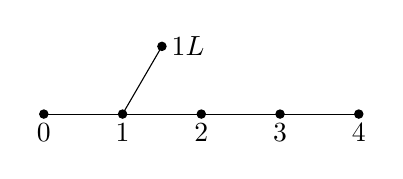
\begin{tikzpicture}
	\draw (0,0) node[anchor=north]{$0$} -- (1,0) node[anchor=north]{$1$} -- (2,0) node[anchor=north]{$2$} -- (3,0) node[anchor=north]{$3$} -- (4,0) node[anchor=north]{$4$};
	\draw (1,0) -- (1.5,0.86) node[anchor=west]{$1L$};
	
	\filldraw[black] (0,0) circle (1.5pt);
	\filldraw[black] (1,0) circle (1.5pt);
	\filldraw[black] (2,0) circle (1.5pt);
	\filldraw[black] (3,0) circle (1.5pt);
	\filldraw[black] (4,0) circle (1.5pt);
	\filldraw[black] (1.5,0.86) circle (1.5pt);
\end{tikzpicture}\\
\end{center}

Caterpillars are also bipartite graphs. That also means it would be relatively easy to compute their nim-values. The graph above is redrawn in the following way to make it convincing that it is, indeed, a bipartite graph.\\

\begin{center}
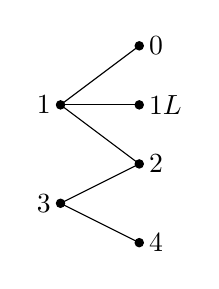
\begin{tikzpicture}
	\draw (1,-0.5) node[anchor=west]{$4$} -- (0,0) node[anchor=east]{$3$} -- (1,0.5) node[anchor=west]{$2$} -- (0,1.25) node[anchor=east]{$1$} -- (1,2) node[anchor=west]{$0$};
	\draw (0,1.25) -- (1,1.25) node[anchor=west]{$1L$};
	
	\filldraw[black] (1,-0.5) circle (1.5pt);
	\filldraw[black] (0,0) circle (1.5pt);
	\filldraw[black] (1,0.5) circle (1.5pt);
	\filldraw[black] (0,1.25) circle (1.5pt);
	\filldraw[black] (1,2) circle (1.5pt);
	\filldraw[black] (1,1.25) circle (1.5pt);
\end{tikzpicture}\\
\end{center}

\begin{theorem}
	\label{caterpillarNimValueTheorem}
	A caterpillar $C_{n,k_1,k_2,...,k_x}$ ($n > 1, 0 < k_1, k_2, ... , k_x < n$) has nim-value $1$ if both $n$ and $x$ have the same parity (both even or odd), otherwise $2$.
\end{theorem}

\begin{proof}
	In a caterpillar $C_{n,k_1,k_2,...,k_x}$, there are $n$ edges in the main path and $x$ edges as legs, i.e., $|E| = n+x$. Also, $|V|=n+x+1$. If $n$ and $x$ have the same parity, $|E|$ is even and $|V|$ is odd, hence it has nim-value $1$. If either of $n$ or $x$ is odd and the other even, $|E|$ is odd and $|V|$ is even, hence it has nim-value $2$.
\end{proof}

\begin{remark}
	Theorem \ref{caterpillarNimValueTheorem} also holds for caterpillars where there are multiple legs at a vertex. 
\end{remark}

Grundy numbers for trees and forests \index{tree} \index{forest} are rather simple to compute. Since tress are bipartite groups, one can use the EV parity. A chomp game on a forest in simply the sum of games on its constituent trees and just like the nim game where the nim-sum is the XOR of the heap sizes, the nim-value of a forest is the XOR of the nim-values of its constituent trees. The following forest has three tress of nim-values $(01)_2$, $(01)_2$ and $(10)_2$. Since $(01)_2 \oplus (01)_2 \oplus (10)_2 = (10)_2$, its nim-value is $2$. Therefore, the winning move in this position is to remove any edge from the third tree which essentially leaves it in a P-position (nim-value $0$).\\

\begin{center}
	\begin{tikzpicture}
	\draw (0,0) -- (0,1) -- (0.707,1.707) -- (0.707,2.707) -- (1.414,3.314);
	\draw (0,1) -- (-0.707,1.707);
	\draw (0.707,2.707) -- (0,3.314);
	
	\filldraw[black] (0,0) circle(1.5pt);
	\filldraw[black] (0,1) circle(1.5pt);
	\filldraw[black] (0.707,1.707) circle(1.5pt);
	\filldraw[black] (-0.707,1.707) circle(1.5pt);
	\filldraw[black] (0.707,2.707) circle(1.5pt);
	\filldraw[black] (1.414,3.314) circle(1.5pt);
	\filldraw[black] (0,3.314) circle(1.5pt);
	
	\draw (3,0) -- (3.707,0.707) -- (4.414,0);
	\draw (3.707,0.707) -- (3.707,1.707) -- (4.414,2.414) -- (4.414,3.414);
	\draw (3.707,1.707) -- (3,2.414);
	
	\filldraw[black] (3,0) circle(1.5pt);
	\filldraw[black] (4.414,0) circle(1.5pt);
	\filldraw[black] (3.707,0.707) circle(1.5pt);
	\filldraw[black] (3.707,1.707) circle(1.5pt);
	\filldraw[black] (4.414,2.414) circle(1.5pt);
	\filldraw[black] (3,2.414) circle(1.5pt);
	\filldraw[black] (4.414,3.414) circle(1.5pt);
	
	\draw (7,0) -- (6.29,0.707) -- (6.29,1.707);
	\draw (7,0) -- (7.707,0.707) -- (7.707,1.707) -- (8.414,2.414);
	
	\filldraw[black] (7,0) circle(1.5pt);
	\filldraw[black] (6.29,0.707) circle(1.5pt);
	\filldraw[black] (6.29,1.707) circle(1.5pt);
	\filldraw[black] (7.707,0.707) circle(1.5pt);
	\filldraw[black] (7.707,1.707) circle(1.5pt);
	\filldraw[black] (8.414,2.414) circle(1.5pt);
	\end{tikzpicture}\\
\end{center}

We have covered nim-values for paths, general caterpillars, 2-regular graphs, trees and forests. We know how to compute nim-values for any bipartite graph. This shall suffice for winning many of the graphs chomps we may likely encounter. However, we still have some more techniques for seemingly complex-looking graphs.

\subsection{Reducible graphs}

Some graphs that look complex can sometimes be rather simple to solve if there is some form of symmetry involved. The graph below is an interesting case. Although it looks random, we can group the vertices into three sets such that it results into three constituent graphs $\{G_1, G_2, G_3\}$. It is easy to see that $G_1$ and $G_2$ are \textit{isomorphic}\index{isomorphic graphs} (this means that they have the same shape and structure and can be transformed to one another by just relabeling the vertices). Further, $G_1$ and $G_2$ are indistinguisable relative to $G_1$ --- for any vertex (or edge) in $G_1$, there is always a corresponding vertex (or edge) in $G_2$. Also, $G_1$ and $G_2$ are not connected by any edge. Such graphs are called reducible graphs.

\begin{center}
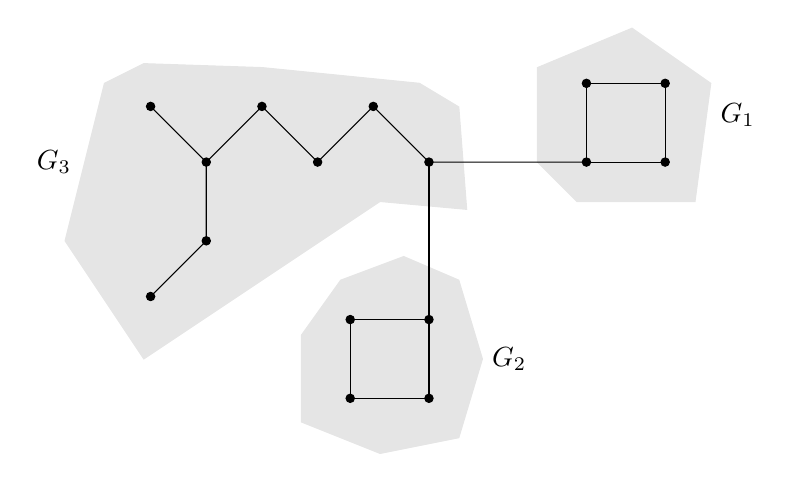
\begin{tikzpicture}
	\filldraw[gray!20] (-1.5,-2.5) -- (0,-1.5) -- (1.5,-0.5) -- (2.6,-0.6) -- (2.5,0.7) -- (2,1) -- (0,1.2) -- (-1.5,1.25) -- (-2,1) -- (-2.5,-1) -- cycle;
	\filldraw[gray!20] (1,-1.5) -- (0.5,-2.2) -- (0.5,-3.3) -- (1.5,-3.7) -- (2.5,-3.5) -- (2.8,-2.5) -- (2.5,-1.5) -- (1.8,-1.2) -- cycle;
	\filldraw[gray!20] (3.5,1.2) -- (3.5,0) -- (4,-0.5) -- (5.5,-0.5) -- (5.7,1) -- (4.7,1.7) -- cycle;
	
	\draw (-2.3,0) node[anchor=east]{$G_3$};
	\draw (2.8,-2.5) node[anchor=west]{$G_2$};
	\draw (5.7,0.6) node[anchor=west]{$G_1$};
	
	
	\draw (-0.707,-1) -- (-0.707,0) -- (0,0.707) -- (0.707,0) -- (1.414,0.707) -- (2.121,0) -- (4.121,0);
	\draw (4.121,0) -- (4.121,1) -- (5.121,1) -- (5.121,0) -- cycle;
	\draw (2.121,0) -- (2.121,-2) -- (2.121,-3) -- (1.121,-3) -- (1.121,-2) -- (2.121,-2);
	\draw (-1.414,0.707) -- (-0.707,0);
	\draw (-0.707,-1) -- (-1.414,-1.707);
	
	\filldraw[black] (-0.707,-1) circle(1.5pt);
	\filldraw[black] (-0.707,0) circle(1.5pt);
	\filldraw[black] (0,0.707) circle(1.5pt);
	\filldraw[black] (0.707,0) circle(1.5pt);
	\filldraw[black] (1.414,0.707) circle(1.5pt);
	\filldraw[black] (2.121,0) circle(1.5pt);
	\filldraw[black] (4.121,0) circle(1.5pt);
	\filldraw[black] (4.121,1) circle(1.5pt);
	\filldraw[black] (5.121,1) circle(1.5pt);
	\filldraw[black] (5.121,0) circle(1.5pt);
	\filldraw[black] (2.121,-2) circle(1.5pt);
	\filldraw[black] (2.121,-3) circle(1.5pt);
	\filldraw[black] (1.121,-3) circle(1.5pt);
	\filldraw[black] (1.121,-2) circle(1.5pt);
	\filldraw[black] (-1.414,0.707) circle(1.5pt);
	\filldraw[black] (-1.414,-1.707) circle(1.5pt);

\end{tikzpicture}\\
\end{center}

Reducible graphs can be reduced to simpler graphs without loss of game information. The graph above, for example, is equivalent to $G_3$. In other words, we need not consider the whole graph; we can remove $G_1$ and $G_2$ and study only $G_3$ without losing anything.

\begin{theorem}
	\label{reducibleGraphTheorem}
	A reducible graph $G=\{G_1,G_2,G_3\}$ where $G_1$ and $G_2$ are isomorphic has the same game position (P or N) as that of the subgraph $G_3$.
\end{theorem}

\begin{proof}
	Suppose Player 1 makes a move on $G_1$, Player 2 can make a corresponding move on $G_2$ such that it remains a reducible graph and $G_3$ is not affected. Any move on $G_2$ can be nullified by a corresponding move on $G_2$ and vice versa. Since the game in finite, both $G_1$ and $G_2$ got exhausted leaving only $G_3$. A move on $G_3$ does not affect either $G_1$ or $G_3$. This implies that any move on the isomorphic subgraphs are just stalling moves (that lengthen or delay the result of the game).
\end{proof}

Using Theorem \ref{reducibleGraphTheorem}, we reduce the graph we considered earlier to $G_3$ without affecting its position (P or N).

\begin{center}
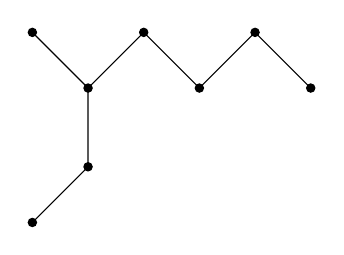
\begin{tikzpicture}
	\draw (-0.707,-1) -- (-0.707,0) -- (0,0.707) -- (0.707,0) -- (1.414,0.707) -- (2.121,0);
	\draw (-1.414,0.707) -- (-0.707,0);
	\draw (-0.707,-1) -- (-1.414,-1.707);
	
	\filldraw[black] (-0.707,-1) circle(1.5pt);
	\filldraw[black] (-0.707,0) circle(1.5pt);
	\filldraw[black] (0,0.707) circle(1.5pt);
	\filldraw[black] (0.707,0) circle(1.5pt);
	\filldraw[black] (1.414,0.707) circle(1.5pt);
	\filldraw[black] (2.121,0) circle(1.5pt);
	\filldraw[black] (-1.414,0.707) circle(1.5pt);
	\filldraw[black] (-1.414,-1.707) circle(1.5pt);
	
\end{tikzpicture}
\end{center}

This is a caterpillar. Using \ref{caterpillarNimValueTheorem}, this has a nim-value 2 --- and therefore, the winning move is to remove any egde leaving it at a P-position.

\begin{remark}
	Theorem \ref{reducibleGraphTheorem} can be generalisted to any number of isomorphic pairs where each isomorphic pair is equivalently connected to the main subgroup. For instance, consider a reducible graph $G=\{G_1,G_2,G_3,G_4,G_5\}$ such that $G_1$ and $G_2$ are isomorphic and equivalently connected to $G_5$ and $G_3$ and $G_4$ are also isomorphic and equivalently connected to $G_5$. The subgraphs $G_1$ and $G_3$ need not be an isomorphic pair. By Theorem \ref{reducibleGraphTheorem} $G$ will have the same position as $G_5$.
\end{remark}


\section{Graph Nim}
\label{graphnim}
\index{graph nim}

\subsection{Nim on graphs}

This is a version of the Nim game which is played on a graph. Consider a graph $G=(V,E)$; a legal move consists of choosing any vertex $v \in V$ and removing any positive number of edges connected to it such that $deg(v)$ decreases to some nonnegative value. The game terminates when there is no legal move left and as with normal play, the player to perfrom the last move wins.\\

Since the rules of the game are general, this can be played on any graph. But we shall look into the cases of some specific types of graphs.

\subsection{Nim on paths}
\index{path graph}

Consider a path graph $P_n$ where $n$ is the number of edges and all vertices have a degree of $2$ but the terminating vertices which have only one connecting edge. We shall follow an indexing system for the vertices where each index $i \in \mathbb{N}\cup\{0\}$ and the leftmost vertex is given an index of $0$.  For a path $P_n$, the vertex indexing set is then $\{0, 1, ..., n\}$. The edge indexing works the same way starting from $0$ (the leftmost edge) and going up to $n-1$ (the rightmost edge). The possible moves in this configuration are --- (1). choose any vertex $v_i$ for $i \not\in \{0,n\}$ and remove either or both the edges connected to that vertex, (2). choose any vertex $v_i$ for $i \in \{0,n\}$ and remove the only connecting edge. For move (1), if $i \not\in \{1, n-1\}$, it results into a disconnected graph containing two path graphs, otherwise it's still a path graph of shorter length. For move (2), the resulting position is always $P_{n-1}$ (ignoring the isolated vertex, of course).

\begin{theorem}
	Nim on a path graph $P_n$ ($n > 0$) is always a first player win.
\end{theorem}

\begin{proof}
	The proof is trivial. For a starting path $P_n$, if $n$ is odd, the winning strategy is this: take out the edge $e_k \in E$, where $k = (n-1)/2$ (this is the middle edge); this leaves two paths of equal sizes $P_{(n-1)/2}$; then mirror any move made by the opponent to leave the game always in symmetry, which is two path graphs of equal sizes. Since the game cannot go on infinitely, it terminates with a graph of no egdes. If $n$ is even, one can take out the two edges connected to $v_{n/2}$ (this is the middle vertex), thus leaving two paths of equal sizes. The situation is similar as above.
\end{proof}

\subsection{Nim on regular graphs}
\index{regular graph}

Consider a 2-regular graph $^2 R_n$. There are $n$ vertices and each vertex has degree 2, i.e., it is an $n$-gon. A legal move is choosing any vertex and taking out either or both the edges. After the first move, the graph turns into a path graph $P_{(n-1)}$ or $P_{(n-2)}$. Therefore, we have instantly arrived at the following theorem.

\begin{theorem}
	\label{regularGraphTheorem}
	Nim on a $2$-regular graph $^2 R_n$ ($n>2$) is always a second player win.
\end{theorem}

\begin{proof}
	The proof is, once again, trivial. Since the path graph nim is a first player win, the second player of the regular graph nim can always use the winning strategy. This is true because the position is a path graph for any move by the first player.
\end{proof}

Having solved the cases of path graphs and 2-regular graphs, we shall now consider the following 3-regular graph with 4 vertices. The idea is to reduce this to a problem whose solution we already have. If we can somehow reduce this to the case of the path graph or the 2-regular graph, then we have solved the problem.\\

\begin{center}
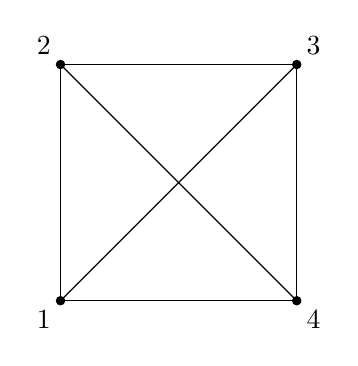
\begin{tikzpicture}
\draw (0,0) node[anchor=north east]{$1$} -- (0,3) node[anchor=south east]{$2$} -- (3,3) node[anchor=south west]{$3$} -- (3,0) node[anchor=north west]{$4$} -- cycle;
\draw (0,0) -- (3,3);
\draw (3,0) -- (0,3);

\filldraw[black] (0,0) circle (1.5pt);
\filldraw[black] (3,0) circle (1.5pt);
\filldraw[black] (0,3) circle (1.5pt);
\filldraw[black] (3,3) circle (1.5pt);
\end{tikzpicture}
\end{center}

The above problem has an easy solution. One can take any vertex and remove all edges connected to it, thus leaving the 2-regular graph $^2 R_3$. Then we use Theorem \ref{regularGraphTheorem} to establish that the problem in hand is a first player win or the 3-regular graph with 4 vertices is an N-position.

\section{Conclusion}

Poset games can be treated as combinatorial games on graphs. Nim, for example, is a chomp on graph. Sprague-Grundy theorem and the mex rule let us to compute Grundy numbers, which help in characterising P-positions and N-positions. Symmetry often simplify games, which might otherwise require more complicated mathematical tools.



\begin{thebibliography}{4}
	\bibitem{winningways}
	E. R. Berlekamp, J. H. Conway, and R. K. Guy.
	\textit{Winning Ways for Your Mathematical Plays}. 2nd ed.
	A K Peters, Ltd., Wellesley, MA (2001).
	
	\bibitem{chomps_on_graphs_and_subsets}
	T. Khandhawit and L. Ye.
	\textit{Chomps on Graphs and Subsets}.
	Available at: \url{https://arxiv.org/pdf/1101.2718.pdf}
	
	\bibitem{broadScientific}
	S. Magura, V. Pong, E. Cartee and K. Valakuzhy.
	\textit{Chomp the Graph}.
	Available at: \url{https://people.eecs.berkeley.edu/~vitchyr/chomp_the_graph.pdf}
	
	\bibitem{daniel_mark}
	J. D. Christensen and M. Tilford.
	\textit{David Gale's Subset Take-Away Game}.
	American Mathematical Monthly 104 (1997), 762-766.
	
	\bibitem{graphicalnim}
	N. J. Calkin, K. James, J. E. Janoski, S. Leggett, B. Richards, N. Sitaraman, S. Thomas.
	\textit{Computing Strategies for Graphical Nim}.
	Available at: \url{https://www.researchgate.net/publication/262449248_Computing_strategies_for_graphical_Nim}
	
	\bibitem{cornellchomp}
	\textit{How to play Chomp}.
	Mathematics Library, Cornell University. 2021.
	Available at: \url{http://
		pi.math.cornell.edu/ ~mec/2003-2004/graphtheory/chomp/howtoplaychomp.
		html.}
	
	\bibitem{wiki-strategystealing}
	\textit{Strategy-stealing argument}.
	Accessed: 2021-06-22. Wikipedia. 2021.
	Available at: \url{https://
		en.wikipedia.org/wiki/Strategy-stealing_argument.}
	
\end{thebibliography}

\printindex

%\newpage
%\section{Tic-tac-toe}
%\begin{itemize}
%	\item If X starts at the center, O should never make a move at the sides, else X can always force a win by placing at one of the farthest corners from O. The only counter for O to X's start at the % center is making a move at one of the corners and then forcing a draw.
%	\item 
%\end{itemize}

\end{document}